\documentclass{article}
\usepackage{graphicx} % Required for inserting images
\usepackage[export]{adjustbox}

\title{Assignment 6: Using the Nagel-Schreckenberg model to investigate traffic patterns on the R44 in Stellenbosch}
\author{Zander Vermeulen}
\date{13 November 2023}

%TODO images out the wazoo

\begin{document}

\maketitle

\section*{Introduction}

The aim of this project was to adapt and expand the model proposed in (Nagel \& Schrekenberg, 1992) to model traffic flow (specifically, southbound traffic during evening peak hours) on and around the R44 between Merriman avenue and the Y-junction with the R310. Data from Google Maps as well as the author's personal experience shows that this is one of the most congested road segments in Stellenbosch (fig. 1). This model could then be used to evaluate strategies employed by road users in an attempt to circumvent this traffic, as well as considering infrastructure changes that could ameliorate the situation.

This project proceeded in multiple phases. At first, the original Nagel-Schreckenberg model was only slightly adjusted to model a linear road segment. Phase 2 involved the addition of junctions along this road segment, while phase 3 considered the effects of traffic lights. In phase 4, the strategy of using Du Toit street to bypass traffic was evaluated, and phase 5 examined the effects that having multiple lanes has on traffic flow, as well as the effects of adding/removing lanes.

All the code, data and resources used in this project is available on GitHub at: https://github.com/theFroodyOne/Physics344Assignment6

\begin{figure}
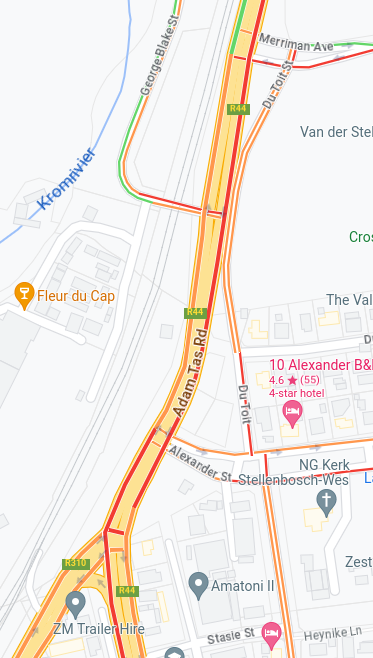
\includegraphics[scale = 0.75]{images/road.png}
\caption{\label{fig} The roads in question. Red shading indicated the slowest traffic, whereas green indicates the fastest. Data shows typical traffic on a Monday evening at 5 pm. Image credit: (Google, 2023a)}
\end{figure}

\section*{Phase 1: Simple model on a linear road segment}

\subsection*{The model}

For phase 1, the model stuck closely to the original proposal in (Nagel \& Schrekenberg, 1992), albeit with different boundary conditions that better reflect the reality of the road in question. In this model, a vehicle appears at the start(north) end of the road with a certain probability $q$ (provided the first cell is unoccupied). $p$ and $v$ have the same interpretation as in the original model, i.e. the probability of a vehicle randomly decelerating and the top speed for all vehicles respectively. The final variable is the length of the road $l$, in cells. The main observable of interest is the number of time-steps a vehicle spends on the road, on average.

\subsection*{Implementation}

This model was implemented in Java (see src/main/java/SimpleModel.java) this creates a class that can be instantiated using the four independent variables in the model at this phase: $q$, $p$, $v$ and $l$. One instantiated, the simulation can be run for single time-step at a time (using \texttt{step()}) or for any number of time-steps (using \texttt{run(int numSteps)}, which returns the average number of time-steps a vehicle spent on the road in that run).

To obtain some exploratory data, $1000$ simulations were run with values of $q \in \{0.1, ... , 1\}$, $p \in \{0, ... , 0.9\}$, $v \in \{3, 6, 9, 12\}$ and $l \in \{5, 10, 20, 40, 80\}$ for $10000$ time-steps, and the average number of time-steps a vehicle spends on the road (time on road, TOR) was recorded (data/phase1/data.csv). This data was then analysed using numpy and matplotlib in dataAnalysis.ipynb. The coefficient of determination $r^{2}$ was calculated between every independent variable and TOR. For more detailed information, the coefficient of determination was also calculated for selected subsets of the data (e.g. effect of $v$ when $p$ is low).

\subsection*{Results}

Unsurprisingly, the largest $r^{2}$ value was observed for $l$, the length of the road in cells, at 40.40\%. $p$ also had a significant effect on TOR, at 27.73\%. Interestingly, the overall effect of $q$ and $v$ was quite low, both with $r^{2}$ less than 1\% (0.8840\% and 0.9128\% respectively). For $p \leq 0.2$, $v$ had a slightly larger effect at 7.239\%. Conversely, $q$ has slightly more effect at higher $p$, 2.824\% for $p \geq 0.8$. Furthermore, when looking at low $p$ regimes, $r^{2}$ for $p$ itself is much lower, just 0.4989\% for $p \leq 0.2$ and 4.746\% for $p \leq 0.5$.

Since $l$ has such a dominating effect, observations were also made with $l$ fixed at 80. $p$ then became the dominating variable (58.70\%), with $v$ having a dominating effect when $p \leq 0.2$ (74.03\%) (fig. 3) and $q$ when $p \geq 0.8$ (73.57\%) (fig. 4).

\begin{figure}
\textbf{\large Average TOR as a function of $p$, with fixed $l=80$}\par\medskip
\rotatebox{90}{{\hspace*{3cm}{\large TOR}}}
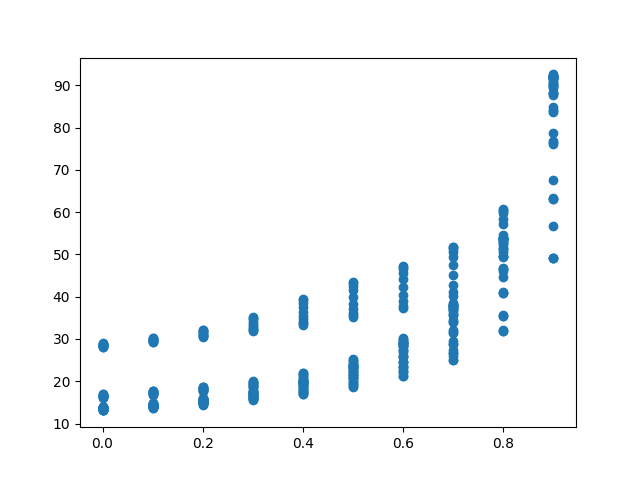
\includegraphics[scale = 0.55, left]{./data/phase1/p_vs_timeOnRoad_l=80.png}
\vspace*{0.1cm}\hspace*{4.5cm}{\large $p$}
\caption{\label{fig} With $l$ fixed at 80, TOR increases slowly with $p$ at first, but then grows exponentially as $p \to 1$.}
\end{figure}

\begin{figure}
\textbf{\large Average TOR as a function of $v$, with fixed $l=80$ and $p \leq 0.2$}\par\medskip
\rotatebox{90}{{\hspace*{3cm}{\large TOR}}}
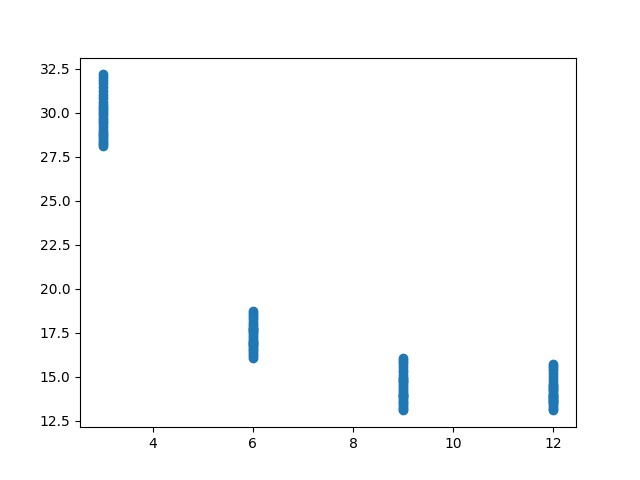
\includegraphics[scale = 0.55, left]{./data/phase1/v_vs_timeOnRoad_l=80_lowp.png}
\vspace*{0.1cm}\hspace*{4.5cm}{\large $p$}
\caption{\label{fig} Looking at low $p$ regimes, the effect of $v$ predominates, i.e. increasing $v$ reduces TOR significantly, albeit with diminishing returns.}
\end{figure}

\begin{figure}
\textbf{\large Average TOR as a function of $q$, with fixed $l=80$ and $p \geq 0.8$}\par\medskip
\rotatebox{90}{{\hspace*{3cm}{\large TOR}}}
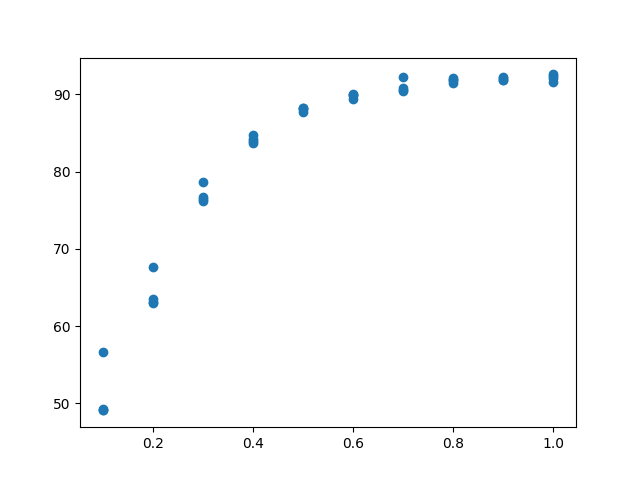
\includegraphics[scale = 0.55, left]{./data/phase1/q_vs_timeOnRoad_l=80_highp.png}
\vspace*{0.1cm}\hspace*{4.5cm}{\large $p$}
\caption{\label{fig} Looking at high $p$ regimes, the effect of $q$ predominates, i.e. more cars on the road slows things down regardless of top speeds.}
\end{figure}

\subsection*{Discussion}

As may be expected, these results indicate that the biggest factor by far influencing TOR is the length of the road. The top speed allowed on the road had a moderate effect when $p$ was low, and $p$ itself only had a large effect when it was quite high ($p \geq 0.5$, unlikely to occur in reality) (this is corroborated by the exponential-looking $p$-TOR curve, fig. 2). Somewhat surprisingly, the effect of $q$ was minimal, meaning that a busy road does not imply slow traffic in this model.

Removing $l$ changed this picture significantly, revealing two possible regimes at low and high $p$ respectively. When $p$ was low, $v$ determined TOR to a high degree, since vehicles were likely to actually reach the top speed when $p$ was low. However, $v$ was mostly irrelevant at high $p$, since vehicles are slowing down randomly too often to ever reach the top speed. In this regime, $q$ largely determined TOR, with a higher inflow of vehicles slowing traffic significantly.

\section*{Phase 2: Inflows and outflows via junctions}

\subsection*{The model}

In this phase, some of the variables had to be nailed down with real-world values to keep the size of the parameter space contained. The road segment in question is approximately 552 meters in length, which, using Nagel \& Schreckenberg's (1992) proposal for cell size (7.5m) this fixes the length of $l$ at 74. Estimating the average acceleration of vehicles on this road as $3m/s^{2}$, this means each time-step corresponds to approximately 2.5s in reality. Furthermore, this implies a maximum speed $v$ of 9 (27 m/s = 97.2 km/h--the true speed limit is 100km/h).

To model the junctions themselves, six more variables were introduced, two for each of the three junctions, namely the probability of a vehicle leaving/joining the R44 at that junction. Vehicles join the R44 simply by appearing at the position of the junction. To be slightly more realistic, the leaving process is somewhat more complex. First, vehicles that will reach/pass a particular junction are identified, and a portion of them are randomly assigned to turn off at the junction according to the leaving probability. These then slow down to reach one cell before the junction by the end of this time-step. Finally, these vehicles "turn off" (i.e. disappear from the model) during the next time-step.

At this point, the model still had 8 variables, all of which could vary independently and continuously between 0 and 1 (since they are all probabilities of some kind). Limiting the range of some of these to values that are physically realistic was therefore necessary to investigate the behaviour effectively. Extrapolating from existing data on traffic flow collected in 2018 (Bredenhann, 2022), reasonable estimates can be made for many of these variables (see table below).

\begin{center}
\begin{tabular}{ |c|c|c| }
 \hline
 Junction & Direction & Probability \\
 \hline
 R44 (i.e. already on road) & Incoming & 0.7736\\
 Merriman & Incoming & 0.7132 \\
 Merriman & Outgoing & 0.3139 \\
 George Blake & Incoming & 0.3938 \\
 George Blake & Outgoing & 0.4007 \\
 Alexander & Incoming & 0.4725 \\
 Alexander & Outgoing & 0.1640 \\
 \hline
\end{tabular}
\end{center}

Data for Alexander Street was not available in (Bredenhann, 2022), so data was collected on the evening of Friday 3 November from 16:20 until around 17:10. Control data was also collected for incoming vehicles on the north end of the R44 so an adjustment could be made for presumed lower traffic volumes on Fridays, and due to the relative dearth of student drivers during the exam period. Traffic flow on the R44 was 85.10\% of those recorded in (Bredenhann, 2022), so volumes recorded on Alexander street were multiplied by a factor of 1.175.

Finally, using TOR as a metric in this phase would be complicated by the fact that vehicles coming in from different junctions have different lengths of road to cover, and lumping them all together would not yield any insightful results. Therefore, the average speed would be the main metric of interest, from which TOR from each junction can be estimated.

\subsection*{Implementation}

This model was implemented in the \texttt{JunctionModel} class, which is a subclass of \texttt{SimpleModel} used for phase 1. Fields were added for the inflow and outflow probabilities as indictated in the table above, with $v$ and $l$ now fixed to correspond to their real-world values. Furthermore, the \texttt{step()} function had to be updated to mark vehicles that will leave the road at the next junction (which necessitated a \texttt{destination} field to be added to the \texttt{vehicle} class) and to remove these when they reached the junction in question. \texttt{run(int numSteps)} was also updated to record average speeds instead of TOR.

1000 simulations were run for 1440 time-steps each (corresponding to 1 hour in real-world time) for each $p \in \{0, 0.01, ... , 0.49\}$ and the average speed recorded in data/phase2/data.csv.

\subsection*{Results}

Average speeds were on the low end, reflecting real-world traffic conditions. Higher values of $p$ also supress speeds, as may be expected (fig. 5). In the ideal case, when $p=0$, speeds reached $v=1.178$, corresponding to a real-world 12.72km/h, degenerating to $v=0$ when $p=1$ and no vehicle ever moves.

Google maps predicts travel times on the entire stretch from just above Merriman to the R310 to be "typically 3-7 minutes" at 5pm on a Tuesday evening (ie. evening peak hours)(Google 2023b). Combined with the data generated here, this can be used to estimate $p$ on this road segment.

A travel time of 3 minutes implies an average speed of $v=1.022$ and 7 minutes $v=0.4381$, which correspond to $p=0.08$ and $p=0.62$ respectively. The median travel time of 5 minutes corresponds to $p=0.31$.

\begin{figure}
\textbf{\large Average speed as a function of $p$}\par\medskip
\rotatebox{90}{{\hspace*{3cm}{\large $\langle v \rangle$}}}
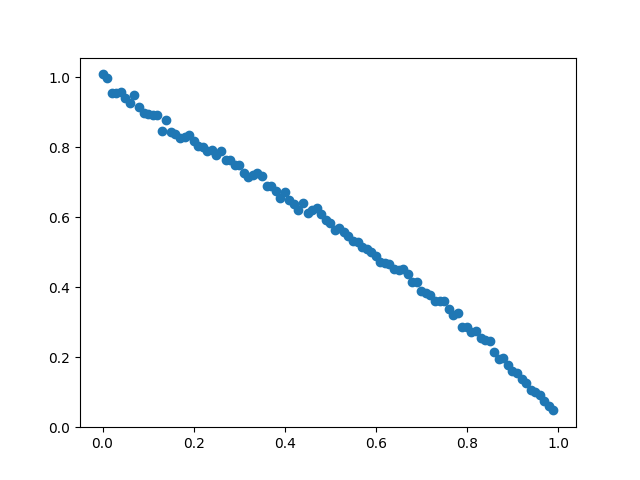
\includegraphics[scale = 0.55, left]{./data/phase2/v_vs_p.png}
\vspace*{0.1cm}\hspace*{4.5cm}{\large $p$}
\caption{\label{fig} Average speeds are low overall due to high congestion, but are even lower at high $p$.}
\end{figure}

\section*{Conclusion}

\section*{References}

%TODO fix alignment of references

Bredenhann, C. (2022). \textit{Stellenbosch Municipality Roads Master Plan: 2022 update}.

Google. (2023a). Retrieved 25 October 2023 from https://www.google.com/maps/@-33.9354554,18.8545061,17z/data=!5m1!1e1?entry=ttu

Google. (2023b). Retrieved 31 October 2023 from https://www.google.com/maps/dir/-33.9325783,18.8529169/-33.9371228,18.8515087/@-33.9349965,18.8496809,17z/data=!4m6!4m5!2m3!6e0!7e2!8j1698771600!3e0?entry=ttu

Nagel, K.; Schreckenberg, M. (1992). "A cellular automaton model for freeway traffic". \textit{Journal de Physique I} 2(12) doi:10.1051/jp1:1992277

\end{document}